\subsection{Metodo di Regolarizzazione di Tikhonov}
Per ridurre gli effetti del rumore nella ricostruzione è necessario introdurre un termine di regolarizzazione di Tikhonov. 

Si considera quindi il seguente problema di ottimizzazione:

Si deve risolvere $Ax_\epsilon = b_\epsilon$ con $b_\epsilon = b+\epsilon$. 
Al posto di risolvere direttamente il sistema lineare (se il sistema è quadrato) o di minimizzare la norma 2 del residuo 
(se il sistema è rettangolare)  $||Ax_\epsilon -b_\epsilon||_2^2$, %! davvero dobbiamo mettere la formula?!

si aggiunge un vincolo di regolarità alla soluzione e si minimizza, ad esempio 
\[||Ax_\epsilon-b_\epsilon||_2^2+\gamma_\epsilon||x_\epsilon||_2^2\] che rappresenta la \textbf{forma standard} 
della regolarizzazione di Tikhonov.

\subsubsection{Immagini geometriche regolarizzate}
Analizziamo i grafici ottenuti cercando di ridurre il rumore nella ricostruzione delle immagini del dataset. 

Grafici andamento PSNR, media PSNR e MSE nella ricostruzione delle immagini con il metodo di regolarizzazione

\begin{figure}[H]
    \centering
    \begin{subfigure}{0.5\textwidth}
        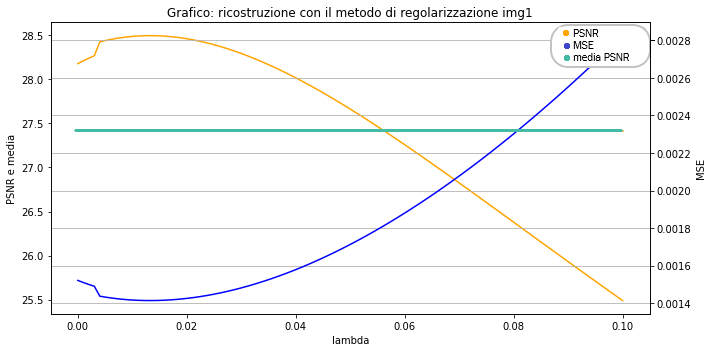
\includegraphics[width=\textwidth]{imgRicostruzione/grafico1minimize.png}
    \end{subfigure}%
    \begin{subfigure}{0.5\textwidth}
        \centering
        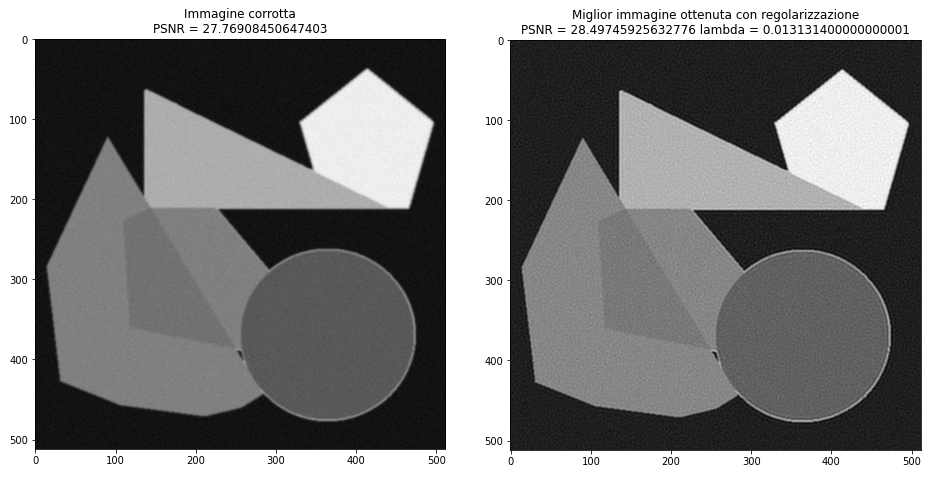
\includegraphics[width=\textwidth]{imgRicostruzione/ricostruzione1minimize.png}
    \end{subfigure}
    \caption{Ricostruzione immagine geometrica img1.png [a destra: immagine corrotta, sinistra: miglior immagine ottenuta con regolarizzazione]}
    
    \begin{subfigure}{0.5\textwidth}
        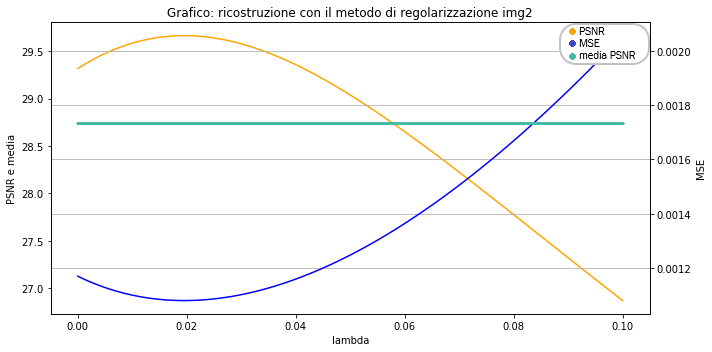
\includegraphics[width=\textwidth]{imgRicostruzione/grafico2minimize.png}
    \end{subfigure}%
    \begin{subfigure}{0.5\textwidth}
        \centering
        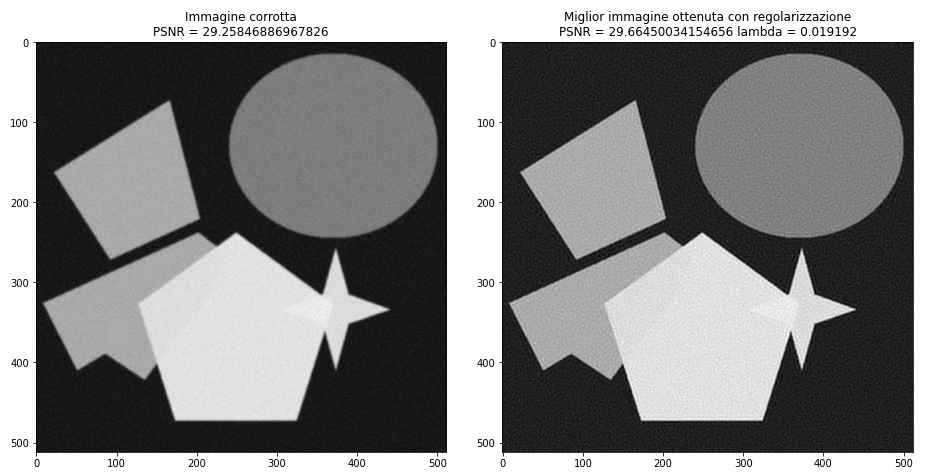
\includegraphics[width=\textwidth]{imgRicostruzione/ricostruzione2minimize.png}
    \end{subfigure}
    \caption{Ricostruzione immagine geometrica img2.png [a destra: immagine corrotta, sinistra: miglior immagine ottenuta con regolarizzazione]}
    
    \begin{subfigure}{0.5\textwidth}
        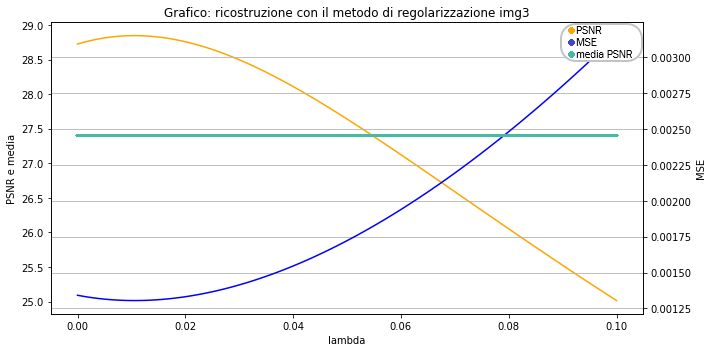
\includegraphics[width=\textwidth]{imgRicostruzione/grafico3minimize.png}
    \end{subfigure}%
    \begin{subfigure}{0.5\textwidth}
        \centering
        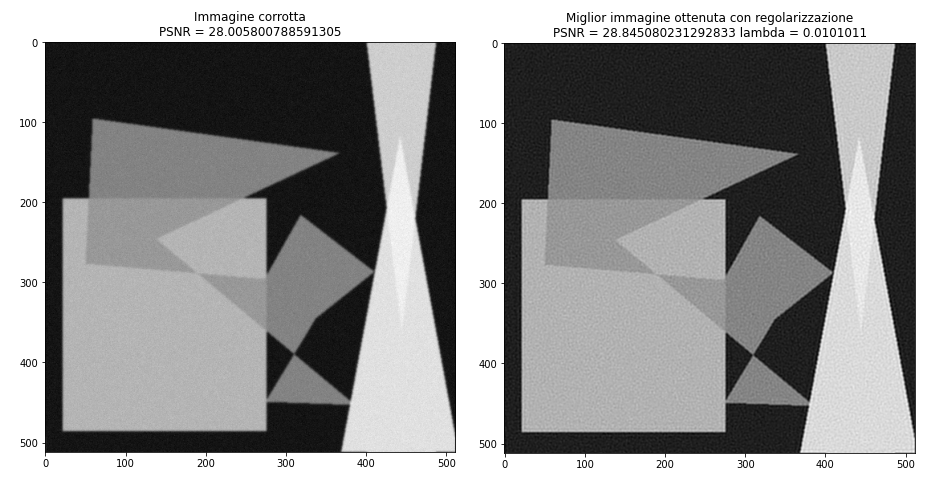
\includegraphics[width=\textwidth]{imgRicostruzione/ricostruzione3minimize.png}
    \end{subfigure}
    \caption{Ricostruzione immagine geometrica img3.png [a destra: immagine corrotta, sinistra: miglior immagine ottenuta con regolarizzazione]}

    \begin{subfigure}{0.5\textwidth}
        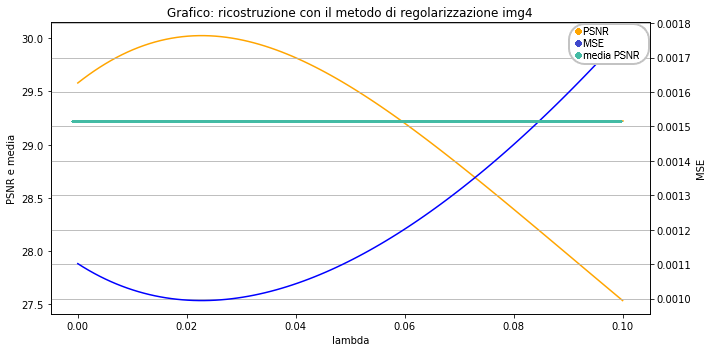
\includegraphics[width=\textwidth]{imgRicostruzione/grafico4minimize.png}
    \end{subfigure}%
    \begin{subfigure}{0.5\textwidth}
        \centering
        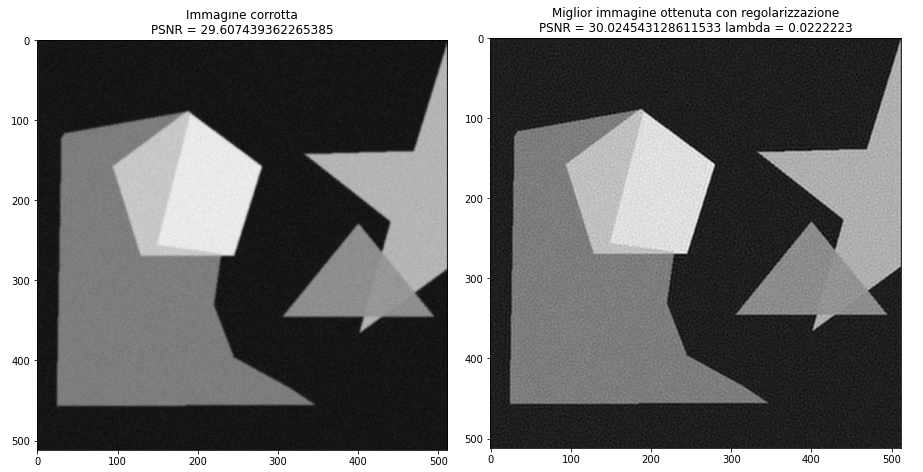
\includegraphics[width=\textwidth]{imgRicostruzione/ricostruzione4minimize.png}
    \end{subfigure}
    \caption{Ricostruzione immagine geometrica img4.png [a destra: immagine corrotta, sinistra: miglior immagine ottenuta con regolarizzazione]}
\end{figure}
\begin{figure}[H]
    \centering
    \begin{subfigure}{0.5\textwidth}
        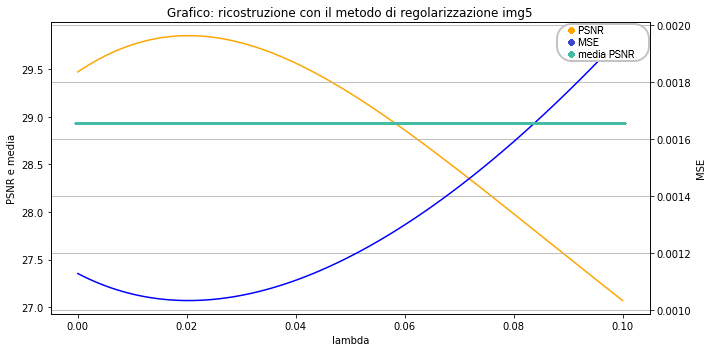
\includegraphics[width=\textwidth]{imgRicostruzione/grafico5minimize.png}
    \end{subfigure}%
    \begin{subfigure}{0.5\textwidth}
        \centering
        
\includegraphics[width=\textwidth]{imgRicostruzione/ricostruzione5minimize.png}
    \end{subfigure}
    \caption{Ricostruzione immagine geometrica img5.png [a destra: immagine corrotta, sinistra: miglior immagine ottenuta con regolarizzazione]}
    
    \begin{subfigure}{0.5\textwidth}
        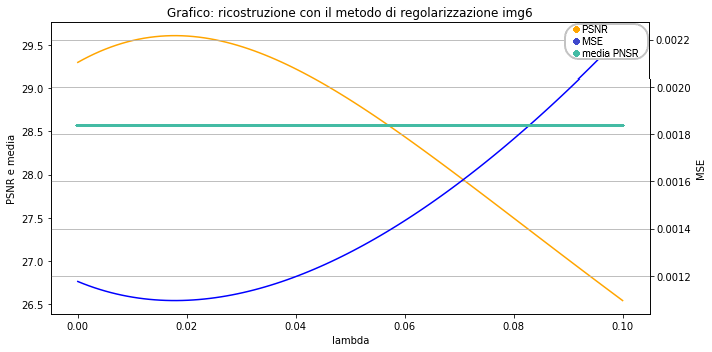
\includegraphics[width=\textwidth]{imgRicostruzione/grafico6minimize.png}
    \end{subfigure}%
    \begin{subfigure}{0.5\textwidth}
        \centering
        
\includegraphics[width=\textwidth]{imgRicostruzione/ricostruzione6minimize.png}
    \end{subfigure}
    \caption{Ricostruzione immagine geometrica img6.png [a destra: immagine corrotta, sinistra: miglior immagine ottenuta con regolarizzazione]}
    
    \begin{subfigure}{0.5\textwidth}
        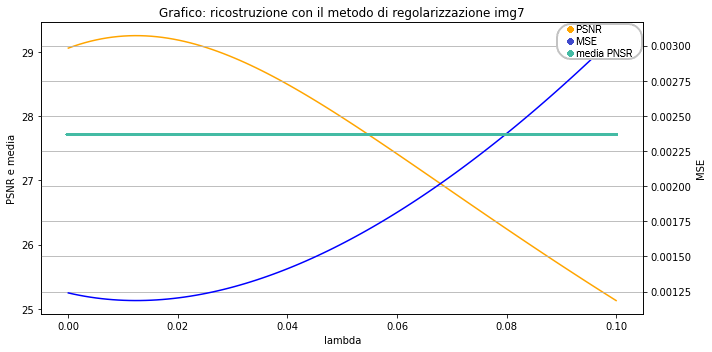
\includegraphics[width=\textwidth]{imgRicostruzione/grafico7minimize.png}
    \end{subfigure}%
    \begin{subfigure}{0.5\textwidth}
        \centering
        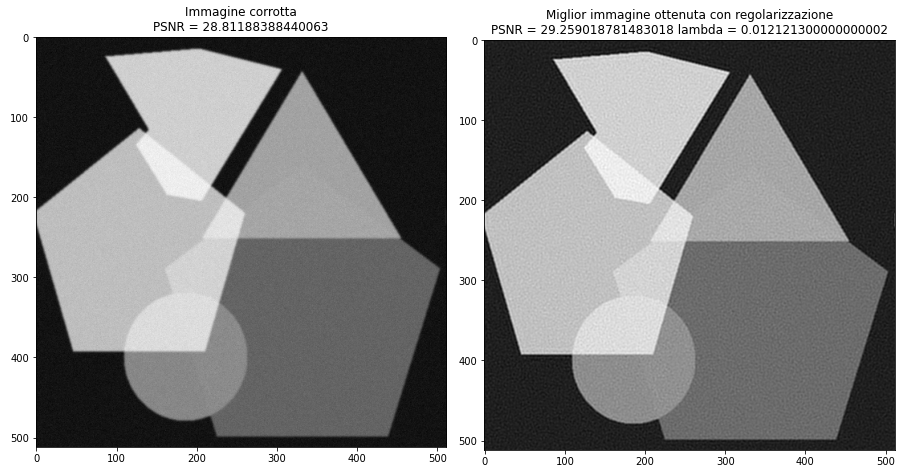
\includegraphics[width=\textwidth]{imgRicostruzione/ricostruzione7minimize.png}
    \end{subfigure}
    \caption{Ricostruzione immagine geometrica img7.png [a destra: immagine corrotta, sinistra: miglior immagine ottenuta con regolarizzazione]}

    \centering
    \begin{subfigure}{0.5\textwidth}
        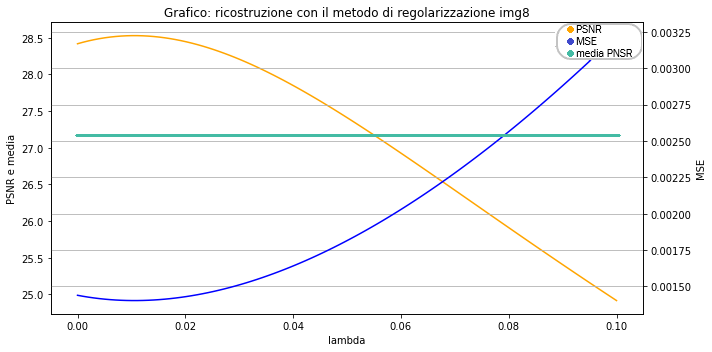
\includegraphics[width=\textwidth]{imgRicostruzione/grafico8minimize.png}
    \end{subfigure}%
    \begin{subfigure}{0.5\textwidth}
        \centering
        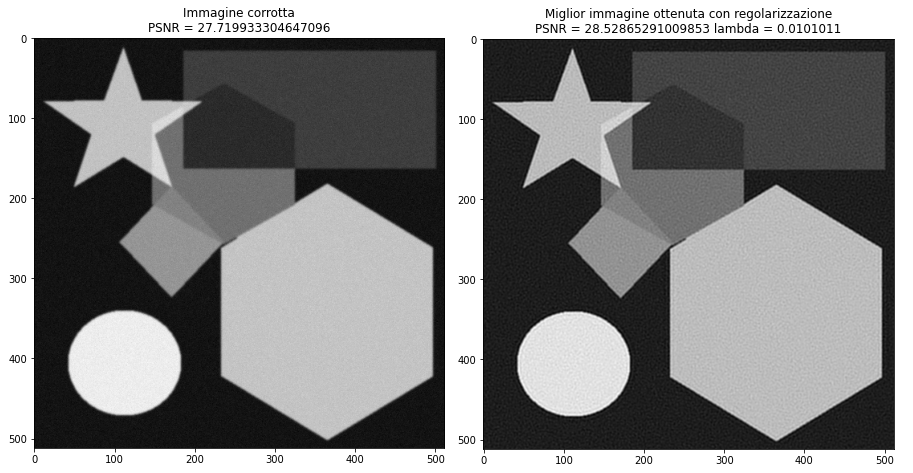
\includegraphics[width=\textwidth]{imgRicostruzione/ricostruzione8minimize.png}
    \end{subfigure}
    \caption{Ricostruzione immagine geometrica img8.png [a destra: immagine corrotta, sinistra: miglior immagine ottenuta con regolarizzazione]}
\end{figure}

\subsubsection{Immagini fotografiche regolarizzate}
\begin{figure}[H]
    \centering
    \begin{subfigure}{0.5\textwidth}
        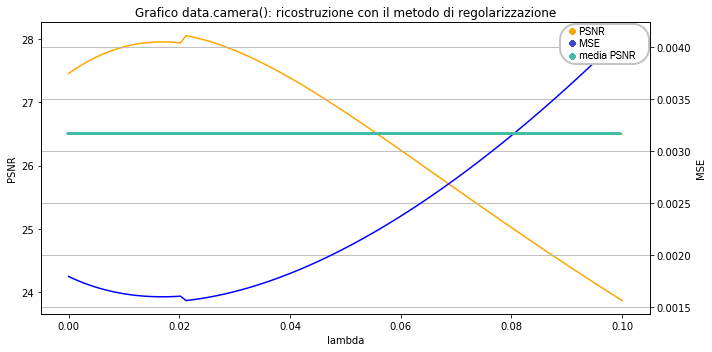
\includegraphics[width=\textwidth]{imgRicostruzione/graficoCameraman_minimize.png}
    \end{subfigure}%
    \begin{subfigure}{0.5\textwidth}
        \centering
        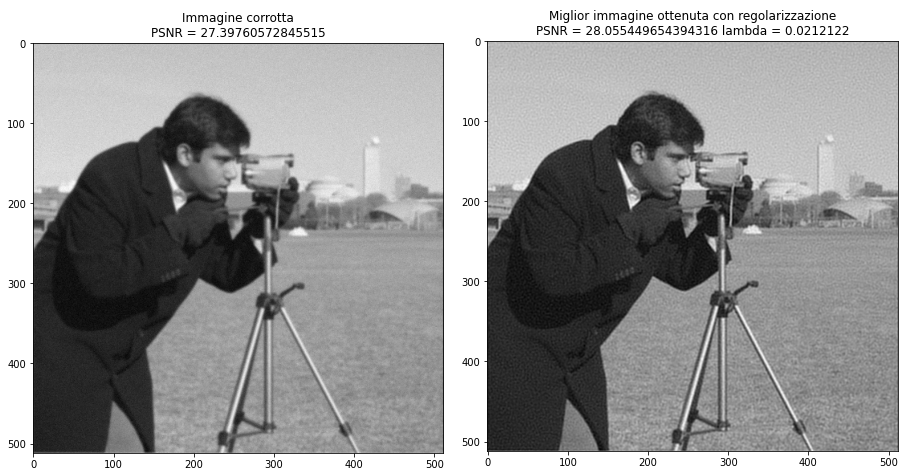
\includegraphics[width=\textwidth]{imgRicostruzione/ricostruzioneCameraman_minimize.png}
    \end{subfigure}
    \caption{Ricostruzione immagine fotografica data.camera() [a destra: immagine corrotta, sinistra: miglior immagine ottenuta con regolarizzazione]}
    
    \centering
    \begin{subfigure}{0.5\textwidth}
        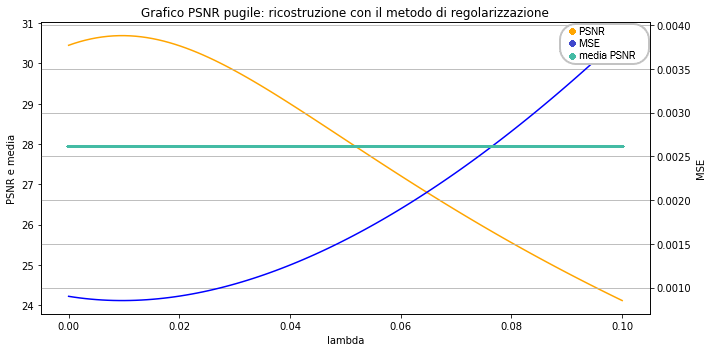
\includegraphics[width=\textwidth]{imgRicostruzione/graficoPugile_minimize.png}
    \end{subfigure}%
    \begin{subfigure}{0.5\textwidth}
        \centering
        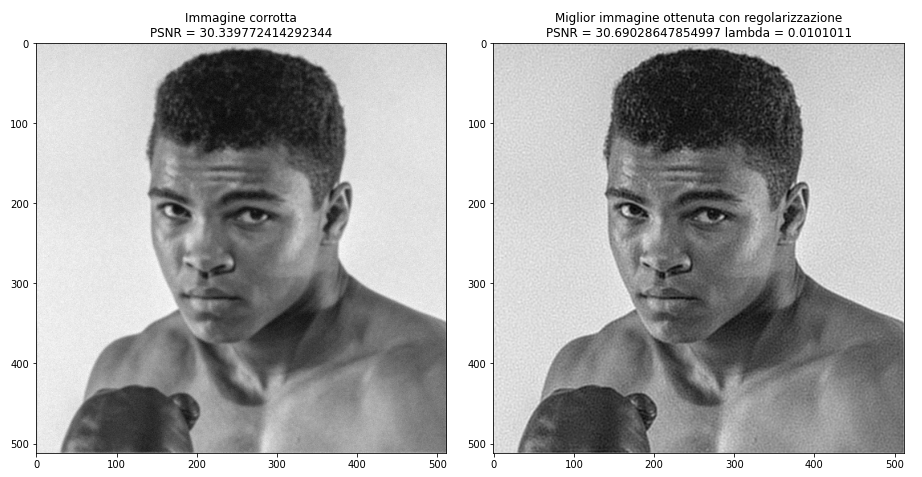
\includegraphics[width=\textwidth]{imgRicostruzione/ricostruzionePugile_minimize.png}
    \end{subfigure}
    \caption{Ricostruzione immagine fotografica pugile.png [a destra: immagine corrotta, sinistra: miglior immagine ottenuta con regolarizzazione]}
    
    \centering
    \begin{subfigure}{0.5\textwidth}
        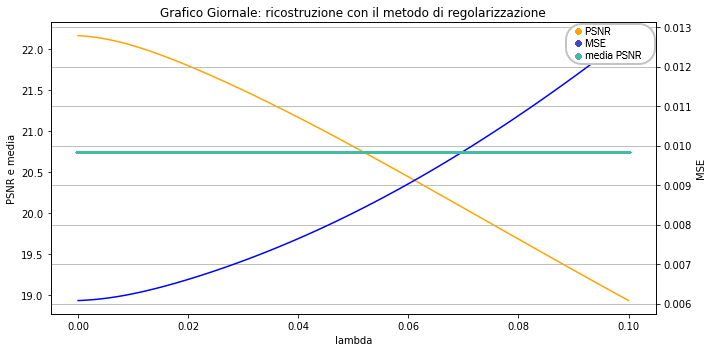
\includegraphics[width=\textwidth]{imgRicostruzione/graficoGiornale_minimize.png}
    \end{subfigure}%
    \begin{subfigure}{0.5\textwidth}
        \centering
        
\includegraphics[width=\textwidth]{imgRicostruzione/ricostruzioneGiornale_minimize.png}
    \end{subfigure}
    \caption{Ricostruzione immagine fotografica giornale.png [a destra: immagine corrotta, sinistra: miglior immagine ottenuta con regolarizzazione]}
\end{figure}